The gain achieved using the Oracular Patent Query method motivates us to explore various methods to approximate the terms
selected by this query without ``peeking at the answers'' provided by
the actual relevance judgements.  We first attempt this via fully
automated methods and then proceed to evaluate semi-automated methods
based on interactive relevance feedback methods.

\subsection{Automated Reduction}
\label{sec:AutomatedReduction}
%\vspace*{-2ex}
%We noticed that most of the useful feedback terms exist in the original query and hypothesized that the baseline system could be substantially improved by removing negative query terms. 
%
% Why these approaches? provide citations for who has suggested them or otherwise
% provide a justification as to why each approach would be a good idea.  Do this
% in the bullet points where the actual method is discussed... not after the bullet
% points!  Don't dissociate content and discuss it multiple times in different
% places!  -Scott
We use the following four simple approaches to reduce the initial patent queries: 
%(i) removing Document Frequent terms (IDF(t)>$\tau$), (ii) keeping Frequent Terms in Query (QTF(t)>$\tau$); (iii) using Pseudo Relevance Feedback set (constructed after an initial run of the query) to select query terms (PRF(t)>$\tau$); and (iv) removing general terms in IPC title. 

\vspace*{0.5mm}
% TODO: Must be consistent in either pruning or removing terms --- results should ideally converge to the baseline at 0.
% TODO: Should do simplest comparisons first and not combine pruning approaches.  Even better: evaluate methods mentioned in related work.
\noindent \textbf{(i)} In standard IR approaches, removing terms appearing highly frequently across documents in the collection can improve retrieval effectiveness. Inspired by this fact, after an initial run of the query, we removed terms  with a high average document frequency (DF) over the top-100 documents ($\mathit{DF}(t)>\tau$). As illustrated in Figure \ref{fig:queryreduc}, such pruning significantly hurts performance. DF pruning continues increasing and converges to the baseline when $\tau $ gets larger values. 

\vspace*{0.5mm}
\noindent \textbf{(ii)} Frequent terms inside long and verbose queries are considered important~\cite{maxwell2013compact}. However, we hypothesise that we may improve the effectiveness by removing terms appearing less frequently in the Patent Query. Therefore, we remove terms with the frequency less than the threshold $\tau$ ($QTF(t)<=\tau$ ). The blue line in Figure~\ref{fig:queryreduc} indicates that the performance gets slightly better than the baseline when we remove less frequent terms in Patent Query. As it can be seen the best MAP achieved when $\tau=5$ and it meets the baseline when $\tau=0$. 
%Frequent terms inside long and verbose queries have been shown to be important~\cite{maxwell2013compact}. Hence, we only keep high query TF (QTF) terms ($\mathit{QTF}(t)>\tau$) but remove from this set any document frequent terms ($\mathit{DF}(t)>0.01$). Figure \ref{fig:queryreduc} indicates that this approach performs slightly better than the baseline.

\vspace*{0.5mm}
\noindent \textbf{(iii)} Pseudo Relevance Feedback ($\mathit{PRF}$) is an automated process without user interaction that assumes the top k ranked documents are relevant and the others are irrelevant. We use $\mathit{PRF}$ to select query terms~\cite{maxwell2013compact} --- the same as what we did for Oracular Relevance Feedback system (Section~\ref{Sec:OracularTermSelection}). We assume that top 5 retrieved documents are relevant and the rest are irrelevant, then we calculate $\mathit{PRF}$ score based on this assumption.  
Terms, which have the $\mathit{PRF}$ score higher than the threshold $\tau$ ($PRF(t)>\tau$), are selected from the Patent Query to reformulate a reduced query. Figure~\ref{fig:queryreduc} shows that this approach is also unsuccessful to achieve a notable improvement over the baseline.

%The third query reduction approach is to select query terms using pseudo-relevance feedback ($\mathit{PRF}$)
%~\cite{Baeza-Yates2011, maxwell2013compact}. We calculated a $\mathit{PRF}$ score similar to $\mathit{RF}$ score assuming that the top-k ranked documents are relevant. We selected the query terms which have high $\mathit{PRF}$ score ($\mathit{PRF}(t)>\tau$). As Figure \ref{fig:queryreduc} illustrates, this approach does not notably outperform the baseline. 
%In fact, we could not find any heuristic correlation between  $ PRF(t)$ and $ RF(t)$. 

\vspace*{0.5mm}
\noindent \textbf{(iv)} The titles of classification indicate their intended content by using a single phrase or several related phrases linked together. We used words in IPC titles for each patent query to reduce the query, based on the assumption that they are common to all patents belonging to the same category and may be considered as stop-words. As it can be seen in Figure~\ref{fig:queryreduc} (black line), this approach slightly helps the performance.
%Finally, we used words in IPC title of each patent query to reduce the query, based on the assumption they are common to all patents, which belong to the same category and may be considered as stop-words. In our experiment, we removed the IPC title terms from a selection of frequent query terms ($QTF(t)>5$). We can see in Figure \ref{fig:queryreduc} that the results drop slightly compared to approach (2), where $\tau=5$.
%\noindent \textbf{(1)-} In standard IR approaches, removing terms, appearing a lot in the collection, helps the retrieval effectiveness. Inspired by this fact, after an initial run of the query, we removed terms  with a Document Frequency (DF) in top-100 documents, higher than the threshold $\tau$. However, as illustrated in Figure \ref{fig:queryreduc}, it's clear that this technique significantly hurts the performance ($DF(t)>\tau$).  
%
%\noindent \textbf{(2)-} Intuitivelly, frequent terms inside long and verbose queries are  important~\cite{maxwell2013compact}. Hence, we have  choosen to reduce queries by selecting terms with a frequency higher than a certain threshold $\tau$. The results in Figure \ref{fig:queryreduc} indicate clearly that this simple and naive technique is not adequate ($QTF(t)>\tau$). 
%
%\noindent \textbf{(3)-} The third approach we experiment to reduce the query is based on Pseudo Relevance Feedback ($\mathit{PRF}$)~\cite{Baeza-Yates2011}. $\mathit{PRF}$ is an automated process without user interaction, which assumes the top k ranked documents are relevant. Again, it can be seen in Figure \ref{fig:queryreduc} that the results for query reduction using $\mathit{PRF}$ do not notably outperform the baseline. In fact, we could not find any heuristic correlation between  $ PRF(t)$ and $ RF(t)$. 
%%Reda: Need clearly to be explained!}
%
%\noindent \textbf{(4)-} Finally, we used words in IPC code title of each patent query to reduce the query, based on the assumption that they are common to all patents, which belong to the same category and may be considered as stop-words. However it did not help.

%we hurt the effectiveness by filtering them out.

% The anecdotal results and their implications have to be explained
% much more clearly... what is surprising about them (be specific:
% point out actual terms) and what can you take away from this
% investigation.  -Scott
\vspace*{0.5mm}
% TODO: What is an IPC title?  I don't know that this is... was it discussed?
Figure \ref{fig:anecdotal} shows an anecdotal example for a sample query about an invention related to ``emulsifier'' to help explain why these four approaches \emph{fail}. It shows the raw abstract of the invention, and terms --- top 20 high scored terms --- and their associated $\mathit{RF}$ scores for each approach. IPC title terms are the words appearing in the IPC title and do not have any score.
%\begin{displaymath}\{t| DF(t)/QTF(t)/PRF(t)>10\}\end{displaymath}
It can be seen that the four methods fail clearly to discriminate between useful and noisy terms. As one example, important stemmed terms like ``enzym'' and ``starch'' have been removed by DF pruning approach, which hurts query quality.  As another example, retaining IPC title terms yields more noisy terms than useful terms (19 out of 32, and few of them with a very negative score like ``amylos'' or ``saccharid'').  Overall, while some methods work better than others for query reduction, all methods may retain highly negative terms and results from Section~\ref{sec:baseline_vs_oracular} showed that the inclusion of even slightly negative terms can significantly hurt performance.
%which resulted in bad retrieval performance. 
%Therefore, this may suggest more sophisticated query reduction methods, as the one discussed in the next section.
 

%high scored terms are polluted with the sufficient amount of noise to hurt the retrieval effectiveness. Unfortunately, none of the proposed query reduction approaches for query reduction worked better than the baseline, which leads us to investigate interactive methods for reduction in the next section.

\subsection{Semi-automated Interactive Reduction}

\label{sec:SemiAutomatedInteractiveReduction}

%%%%%%%%%%%%%%%%%%%%%%%%%%%%%%%%%%%%%%%%%%%%%%%%%%%%%%%%%%%%
%\begin{figure}[t!]
%\begin{centering}
%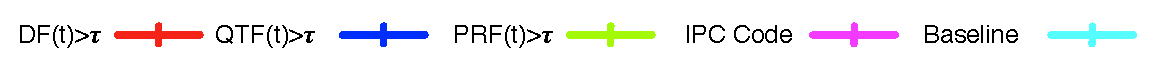
\includegraphics[width=9cm]{imgs/legend2}
%\par\end{centering}
%
%\begin{centering}
%\subfigure[{Mean Average Precision.}]{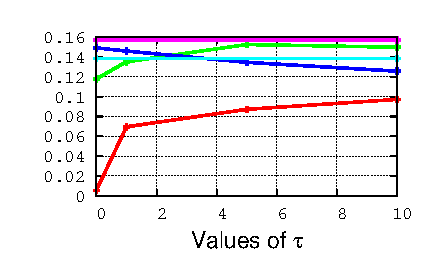
\includegraphics[width=4.5cm]{imgs/figure2-MAP}}\subfigure[Recall.]{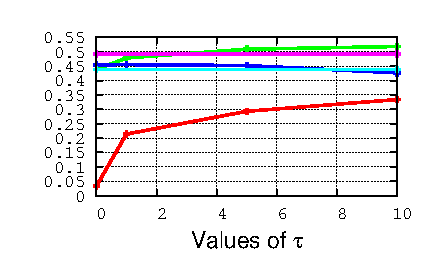
\includegraphics[width=4.5cm]{imgs/figure2-Recall}}
%\par\end{centering}
%
%\protect\caption{System performance vs. the threshold $\tau$ for four query reduction approaches.}
%\label{fig:queryreduc}
%\end{figure}
%%%%%%%%%%%%%%%%%%%%%%%%%%%%%%%%%%%%%%%%%%%%%%%%%%%%%%%%%%%%
%%%%%%%%%%%%%%%%%%%%%%%%%%%%%%%%%%%%%%%%%%%%%%%%%%%%%%%%%%%%
\begin{figure}[t!]
\begin{centering}
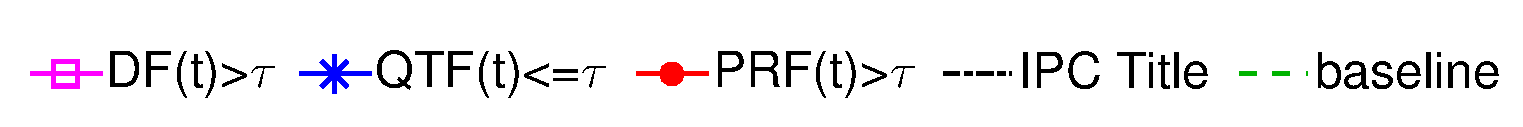
\includegraphics[width=9cm]{imgs/l2.eps}
\par\end{centering}
\begin{centering}
\subfigure[{Mean Average Precision.}]{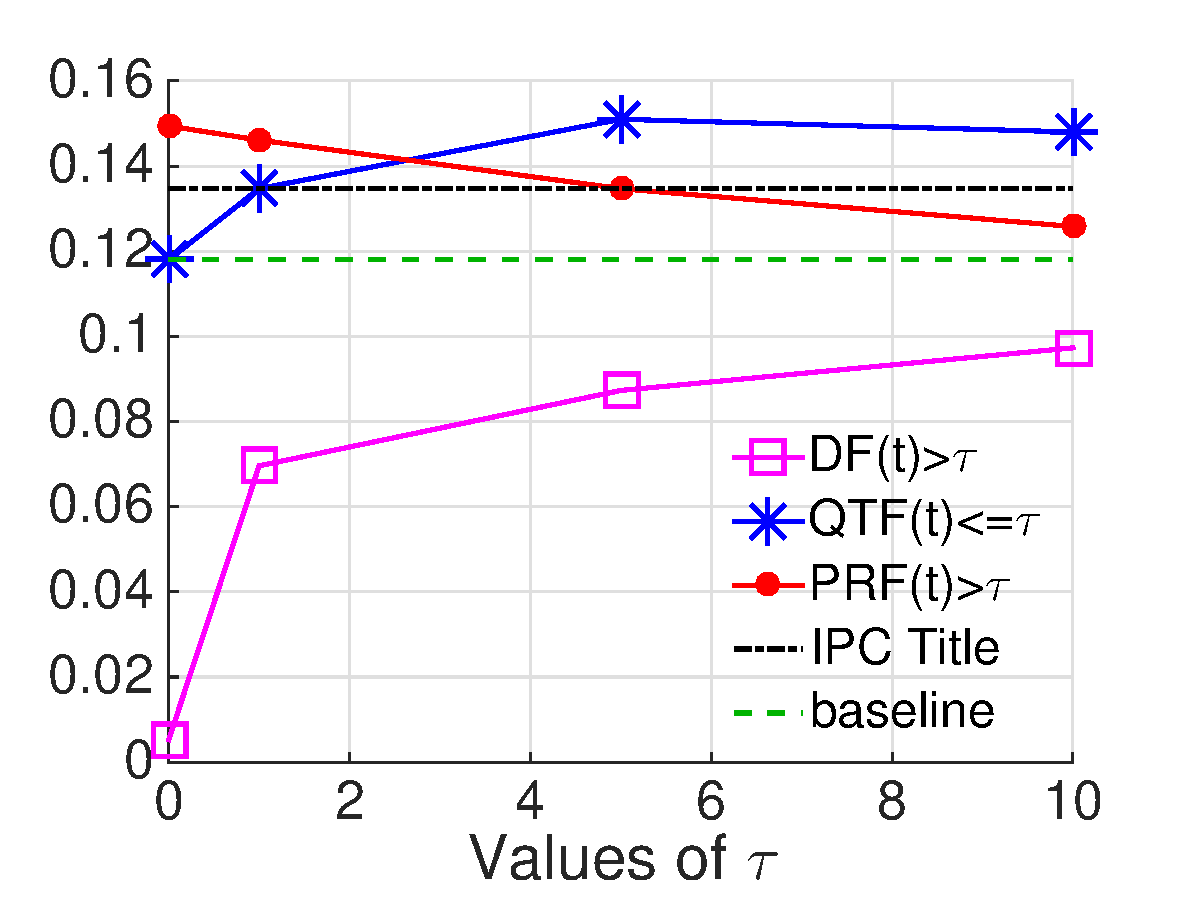
\includegraphics[width=4.5cm, height=3.5cm]{imgs/fig2_map}}\subfigure[Recall.]{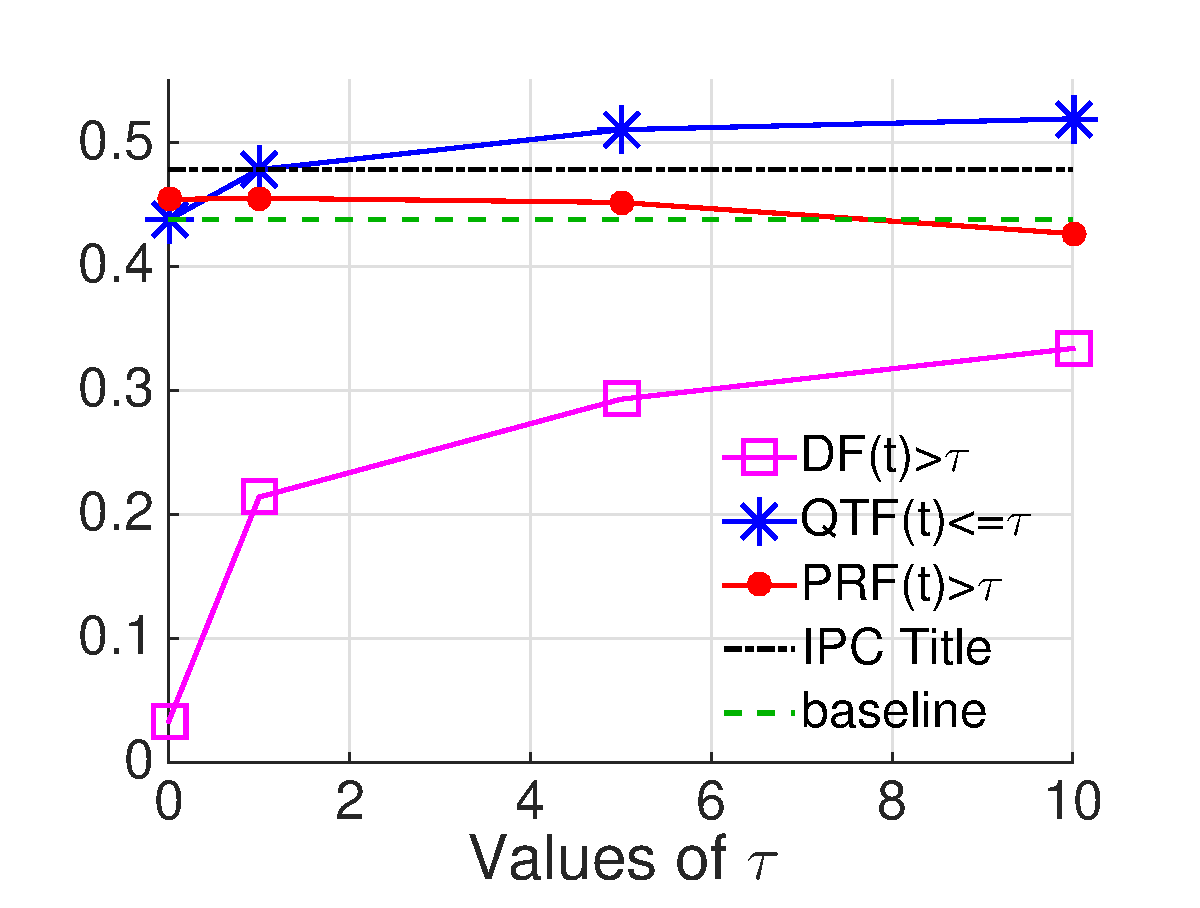
\includegraphics[width=4.5cm, height=3.5cm]{imgs/fig2_recall}}
\par\end{centering}

\protect\caption{System performance vs. the threshold $\tau$ for four query reduction approaches.}
\label{fig:queryreduc}
\end{figure}
%%%%%%%%%%%%%%%%%%%%%%%%%%%%%%%%%%%%%%%%%%%%%%%%%%%%%%%%%%%%
%%%%%%%%%%%%%%%%%%%%%%%%%%%%%%%%%%%%%%%%%%%%%%%%%%%%%%%%%%%%
\begin{figure}[t!]
\begin{framed}
\vspace*{-2ex}
  \centering
    %\lstinputlisting[frame=single, basicstyle=\scriptsize\ttfamily , linewidth=\columnwidth,breaklines=true]{code/anecdotale.tex}\vspace*{-2ex}
 \begin{lstlisting}[basicstyle=\scriptsize\ttfamily , linewidth=\columnwidth,breaklines=true] 
PAC-1293
Abstract: The invention relates to an emulsifier, 
a method for preparing said emulsifier, and to 
its use in various applications, primarily food 
and cosmetic applications. The invention also 
relates to the use of said emulsifier for the 
creation of an elastic, gelled foam. An 
emulsifier according to the invention is based on 
a starch which is enzymatically converted, using 
a specific type of enzyme, and modified in a 
specific esterification reaction.
<@\vspace{-2mm}@>
<@\underline{DF Terms:}@> <@\textcolor{blue}{starch:14.6}@>,<@\textcolor{blue}{enzym:29.5}@>,<@\textcolor{red}{amylos:-20.1}@>,<@\textcolor{blue}{oil:8.6}@>,
<@\textcolor{red}{dispers:-8.7}@>,<@\textcolor{red}{ph:-4.6}@>, <@\textcolor{red}{dry:-6.2}@>,<@\textcolor{red}{heat:-2.3}@>,<@\textcolor{red}{product:-5.5}@>,
<@\textcolor{red}{slurri:-11.5}@>,<@\textcolor{blue}{viscos:7.8}@>,<@\textcolor{red}{composit:-4.5}@>,<@\textcolor{red}{reaction:-2}@>,
<@\textcolor{red}{food:-11.9}@>,<@\textcolor{blue}{agent:5.2}@>,<@\textcolor{red}{debranch:-10.6}@>,<@\textcolor{red}{reduc:-6.4}@>,<@\textcolor{red}{fat:-12.8}@>,
<@\textcolor{red}{prepar:-0.8}@>,<@\textcolor{red}{hour:-5.4}@>
<@\vspace{-2mm}@>
<@\underline{QTF Terms:}@> <@\textcolor{blue}{starch:14.6}@>,<@\textcolor{blue}{emulsifi:6.7}@>,<@\textcolor{red}{succin:-3.5}@>,
<@\textcolor{blue}{enzym:29.5}@>,<@\textcolor{blue}{emuls:12.7}@>,<@\textcolor{blue}{hydrophob:5.4}@>,<@\textcolor{red}{anhydrid:-5.5}@>,
<@\textcolor{red}{reaction:-2}@>,<@\textcolor{red}{octenyl:-0.7}@>,<@\textcolor{blue}{stabil:3.6}@>,<@\textcolor{blue}{alkenyl:0.06}@>,
<@\textcolor{blue}{reagent:1.2}@>,<@\textcolor{blue}{carbon:0.1}@>,<@\textcolor{blue}{potato:3.7}@>,<@\textcolor{red}{alkyl:-0.3}@>,<@\textcolor{red}{wt:-4.6}@>,
<@\textcolor{blue}{ether:2}@>,<@\textcolor{red}{enzymat:-3.4}@>,<@\textcolor{blue}{convers:10.4}@>,<@\textcolor{red}{chain:-5.5}@>
<@\vspace{-2mm}@>
<@\underline{PRF Terms:}@> <@\textcolor{blue}{starch:14.6}@>,<@\textcolor{blue}{encapsul:17.5}@>,<@\textcolor{red}{chees:-4.2}@>,<@\textcolor{blue}{oil:8.6}@>,
<@\textcolor{blue}{hydrophob:5.4}@>,<@\textcolor{blue}{agent:5.2}@>,<@\textcolor{red}{casein:-2.2}@>,<@\textcolor{blue}{degrad:17.1}@>,<@\textcolor{blue}{deriv:12}@>,
<@\textcolor{blue}{tablet:5.3}@>,<@\textcolor{red}{debranch:-10.6}@>,<@\textcolor{red}{imit:-1.1}@>,<@\textcolor{blue}{viscos:7.8}@>,<@\textcolor{blue}{oxid:6}@>,
<@\textcolor{blue}{activ:6}@>,<@\textcolor{blue}{osa:9.3}@>,<@\textcolor{blue}{funnel:2.7}@>,<@\textcolor{blue}{amylas:26.1}@>,<@\textcolor{red}{amylopectin:-7.1}@>,
<@\textcolor{blue}{maiz:20.6}@>
<@\vspace{-2mm}@>
<@\underline{IPC title Terms:}@><@\textcolor{blue}{cosmet:3.8}@>,<@\textcolor{blue}{toilet:0.2}@>,<@\textcolor{red}{prepar:-0.8}@>,
<@\textcolor{blue}{case:0.5}@>,<@\textcolor{red}{accessori:-0.01}@>,<@\textcolor{red}{store:-0.4}@>,<@\textcolor{blue}{handl:0.07}@>,<@\textcolor{red}{pasti:-0.2}@>,
<@\textcolor{red}{substanc:-1.2}@>,<@\textcolor{red}{fibrou:-0.01}@>,<@\textcolor{red}{pulp:-1.3}@>,<@\textcolor{red}{constitut:-0.06}@>,
<@\textcolor{blue}{paper:1.3}@>,<@\textcolor{red}{impregn:-0.1}@>,<@\textcolor{blue}{emulsifi:6.7}@>,<@\textcolor{red}{wet:-0.3}@>,<@\textcolor{red}{dispers:-8.6}@>,
<@\textcolor{red}{foam:-0.5}@>,<@\textcolor{red}{produc:-0.6}@>,<@\textcolor{blue}{agent:5.2}@>
 \end{lstlisting} 
 \vspace*{-2ex}
\end{framed}
 \vspace*{-2ex}
  \caption{Four query reduction approaches on a sample query.  Top
    terms retained by each method are shown.  Numerical oracular
    scores $\mathit{RF}(t,Q)$ are provided indicating whether the term
    was useful (blue/positive) or noisy (red/negative).}
  \label{fig:anecdotal}  
\end{figure}
%%%%%%%%%%%%%%%%%%%%%%%%%%%%%%%%%%%%%%%%%%%%%%%%%%%%%%%%%%%%

Our sample analysis of specific queries and terms selected via our oracular
approach suggests that automated methods fall far short of optimal term selection.
This leads us to explore another approach of approximating the oracular query
derived from relevance judgements by using a subset of relevance judgements
through interactive methods.  Specifically, to minimize the need for user interaction,
in this section we analyse the performance of an oracular query derived from
only the first relevant document identified in the search results.
\begin{comment}
All our attempts to improve the system effectiveness without accessing the relevance feedback were quite in vein because the features we recognized were tightly the combination of the useful words and noisy words and the system performance is too sensitive to the existence of a noisy word or the absence of the useful terms. So, we decided to apply much more realistic approach in which feedback terms are extracted only from the first ranked relevant document retrieved. 
\end{comment}
Using this approach, Table \ref{tab:firstrel} shows that we can double the MAP in comparison to our baseline and also outperform the PATATRAS system.

%%%%%%%%%%%%%%%%%%%%%%%%%%%%%%%%%%%%%%%%%%%%%%%%%%%%%%%%%%%%%%%%
\begin{table}[t!]
  \begin{center}
   \caption{System performance using minimal relevance feedback. $\tau$ is RF score threshold, and $k$ indicates the number of first relevant retrieved patents.}\vspace{3mm}
  \input table/partialRFtermselect.tex   
  \label{tab:firstrel}
  \end{center}  
\end{table}
%%%%%%%%%%%%%%%%%%%%%%%%%%%%%%%%%%%%%%%%%%%%%%%%%%%%%%%%%%%%%%%%

Furthermore, to establish the minimal interaction required by this
approach, Figure \ref{fig:FirstTPRankHisto} indicates that the
baseline methods return a relevant patent approximately 80\% of the
time in the first 10 results and 90\% of the time in the first 20
results.  Hence, such an interactive approach requires relatively low
user effort while achieving state-of-the-art performance.


\begin{figure}
\begin{centering}
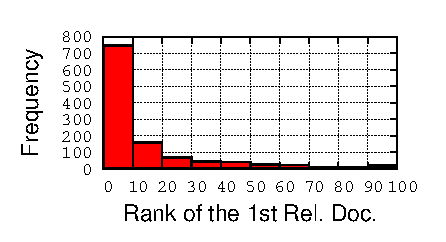
\includegraphics[width=5.5cm]{imgs/1stRank}
\par\end{centering}

\protect\caption{The distribution of the first relevant document rank over test queries.}
\label{fig:FirstTPRankHisto}
\end{figure}


